%\documentclass{article}
\documentclass[twoside, 12pt,a4paper]{article}
% Damit die Verwendung der deutschen Sprache nicht ganz so umst\"andlich wird,
% sollte man die folgenden Pakete einbinden: 
%\usepackage[latin1]{inputenc}% erm\"oglich die direkte Eingabe der Umlaute 
\usepackage[utf8]{inputenc}
\usepackage[T1]{fontenc} % das Trennen der Umlaute
%\usepackage{ngerman}[babel] 
\usepackage[english,ngerman]{babel} %Version in meinem Numerik Vortrag
\usepackage{caption}[2011/11/10]
\newcommand{\figsource}[1]{%
	\addtocounter{figure}{-1}
	\captionlistentry{source: #1}
}
\usepackage{verbatim}
\usepackage[multiple]{footmisc}
\usepackage{pythontex} % \inputpygments{python}{file_1.py}
\usepackage{caption}
\usepackage{verbatim}
\usepackage{subcaption}
\usepackage{amssymb}  
\usepackage{amsmath}
\usepackage{amsthm}
\usepackage{hyperref}
\usepackage{graphicx}
\graphicspath{{images/}} %import images from follder "images

\usepackage{apacite} %bibliography file
\pagenumbering{arabic}
\usepackage{caption}
%\usepackage{ntheorem}
\usepackage{tabto}  
\usepackage{appendix}  
\usepackage[multiple]{footmisc} %multiple footnotes
\newcommand\mytab{\tab \hspace{1cm}}
%\theoremstyle{break}

%%% ------------ Kopf- und Fußzeile
% https://esc-now.de/_/latex-individuelle-kopf--und-fusszeilen/?lang=de
\usepackage[headtopline,headsepline]{scrpage2}
\pagestyle{scrheadings}
\renewcommand{\headfont}{\scriptsize}

\clearscrheadfoot
\ofoot{\pagemark}

\ohead{\headmark}
\automark[subsection]{section}

% Linien

\setheadtopline{0pt}
\setheadsepline{.5pt}

% Keywords command
\providecommand{\keywords}[1]
{
	\small	
	\textbf{\textit{Keywords---}} #1
}
%%% -----------Theorem, Sätze, Beweise ----------------------------------------
%vgl. O.C.Schnürer FA Skript
%\usepackage{amsthm}

\def\emph#1{\textit{#1}}

%\newtheorem{theorem}{Theorem}[chapter]
\newtheorem{theorem}{Theorem}[subsection]
\newtheorem{lemma}[theorem]{Lemma}
\newtheorem{satz}[theorem]{Satz}
\newtheorem{proposition}[theorem]{Proposition}
\newtheorem{corollary}[theorem]{Korollar}

%\theoremstyle{definition}
\newtheorem{definition}[theorem]{Definition}
\newtheorem{example}[theorem]{Beispiel}
\newtheorem{beispiel}[theorem]{Beispiel}
\newtheorem{beispiele}[theorem]{Beispiele}
\newtheorem{xca}[theorem]{\"Ubung}
\newtheorem{notation}[theorem]{Notation}

\newtheorem{aufgabe}{Aufgabe}[section]
%\theoremstyle{remark}
\newtheorem{remark}[theorem]{Bemerkung}
\newtheorem{bemerkung}[theorem]{Bemerkung}
\newtheorem{herleitung}[theorem]{Herleitung}

%\numberwithin{section}{chapter}
%\numberwithin{equation}{chapter}
\numberwithin{equation}{section}

%\renewcommand*{\proofname}{Beweis}
%%% -----------------------------------------------------------
% Python code einfügen:
\usepackage{listings}
\usepackage{xcolor}

\definecolor{codegreen}{rgb}{0,0.6,0}
\definecolor{codegray}{rgb}{0.5,0.5,0.5}
\definecolor{codepurple}{rgb}{0.58,0,0.82}
\definecolor{backcolour}{rgb}{0.95,0.95,0.92}

\lstdefinestyle{mystyle}{
	backgroundcolor=\color{backcolour},   
	commentstyle=\color{codegreen},
	keywordstyle=\color{magenta},
	numberstyle=\tiny\color{codegray},
	stringstyle=\color{codepurple},
	basicstyle=\ttfamily\footnotesize,
	breakatwhitespace=false,         
	breaklines=true,                 
	captionpos=b,                    
	keepspaces=true,                 
	numbers=left,                    
	numbersep=5pt,                  
	showspaces=false,                
	showstringspaces=false,
	showtabs=false,                  
	tabsize=2
}

\lstset{style=mystyle}

%% --------------glossary -----------------------------

\usepackage[toc]{glossaries}

\newglossaryentry{llrp}
{
	name=Layer-wise Relevance Propagation,
	description={Verfahren zur Relevanzverteilung auf einzelne Neuronen eines Neuronalen Netzwerkes}
}

\newglossaryentry{latex}
{
	name=latex,
	description={Is a mark up language specially suited 
		for scientific documents}
}
\newacronym{lrp}{LRP}{Layer-wise Relevance Propagation}
\newacronym{dtd}{DTD}{Deep Taylor-Decomposition}
\newacronym{nn}{NN}{Neuronales Netzwerk}

\makeglossaries

%%-------------bibfile---------------------------------
%\usepackage{apacite}

%%%%%%%%%%%%%%%%%%%% -------------------------------------------------
%\newtheorem{theorem}{Theorem}
\title{Masterarbeit}
\title{\line(1,0){350}\\Untersuchung \& Entwicklung \\von Ansätzen zur Detektion von Poisoning-Angriffen\\\line(1,0){350}\\
	Master-Arbeit}
\author{
	Lukas Schulth\\
	\texttt{lukas.schulth@uni.kn}
}

\date{1. Oktober 2021}

\begin{document}
	\begin{titlepage}
		
		
		
		\thispagestyle{empty} 
		\begin{figure}
			\centering
			\begin{minipage}{0.45\textwidth}
				\centering
				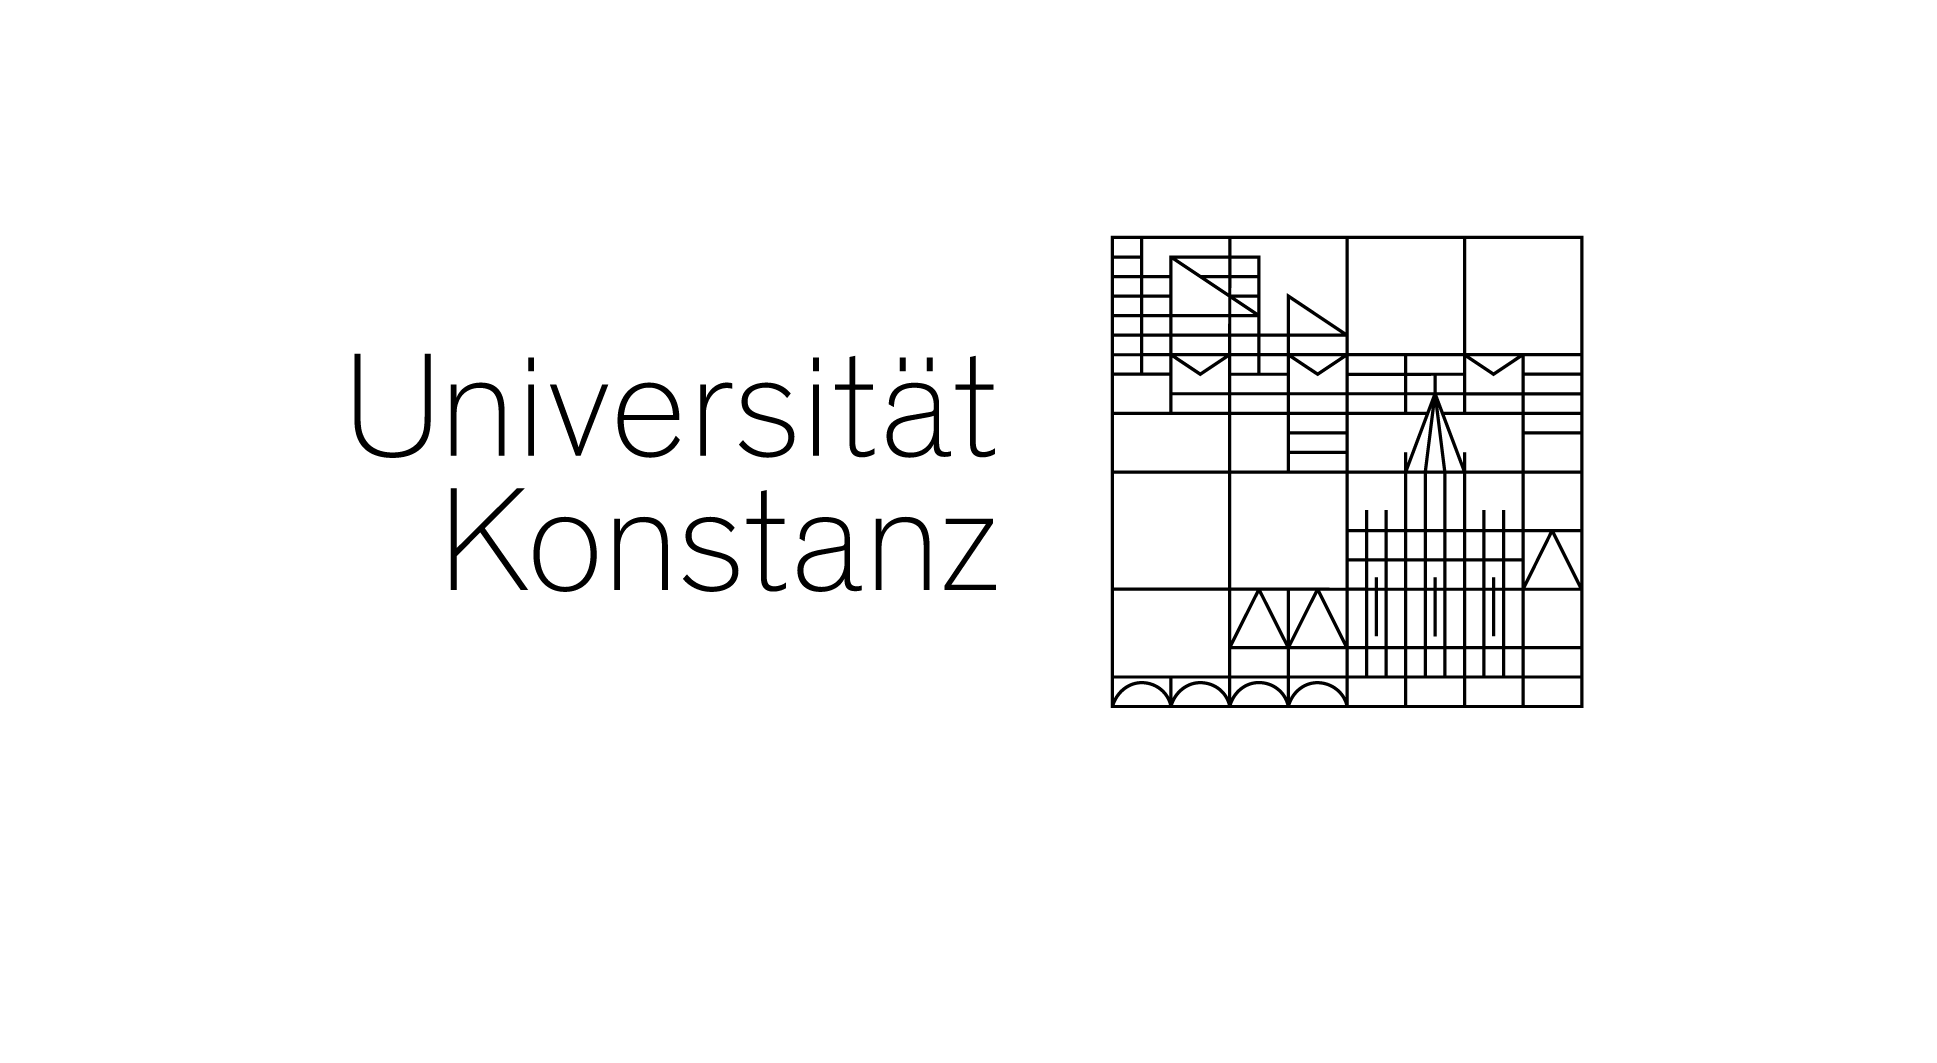
\includegraphics[width=1.2\textwidth]{logounikn} % first figure itself
				
			\end{minipage}\hfill
			\begin{minipage}{0.45\textwidth}
				\centering
				
\includegraphics[width=0.9\textwidth]{bsi_logo} % second figure itself
			
			\end{minipage}
		\end{figure}
	\maketitle
	
	Erstkorrektor, Zweitkorektor, Betreuer, Fachbereich Mathematik und Statistik, Masterarbeit zur Erlangung des Titels Master of Science (M.Sc.)
	
	vgl. mit Titelblatt Exposé(!)
	
	\end{titlepage}
	\selectlanguage{english}
	\begin{abstract}english\end{abstract}
	\selectlanguage{ngerman}
	\begin{abstract}deutsch\end{abstract}

	\keywords{one, two, three, four}
	\newpage
	%\thispagestyle{empty} 
	\listoffigures
	
	\listoftables
	
	\lstlistoflistings
	
	\newpage
	\tableofcontents
	\newpage
	

	
	
	
	\section{Einführung}
	
	A Complete List of All (arXiv) Adversarial Example Papers \footnote{\url{https://nicholas.carlini.com/writing/2019/all-adversarial-example-papers.html}}
	\\
	In sicherheitskritischen Anwendungsgebieten ist die Erklärung für das Zustandekommen einer Entscheidung genauso wichtig wie die Entscheidung selbst\cite{LRP_DNN}.
	
	Clustering auf Datenpunkten direkt(~50 Prozent = raten), Clustering auf Aktivierungen gut geeigneter Netzwerkschichten. Clustering auf den Heatmaps der verdächtigen Klasse.\\
	\\
	
	Clustering auf unterschiedlichen Repräsentationen der Bilder:
	\begin{itemize}
		\item Clustering direkt auf den Bildern\\
		\item Clustering auf den Activations einer Netzwerkschicht(Im Paper \cite{AC} wird die vorletzte Schicht benutzt)
		\item Clustering auf den Heatmaps
	\end{itemize}
	In \autoref{chapter_nn} geben wir eine kurze Einführung in Neuronale Netzwerke und stellen die untersuchten Modelle vor. \autoref{chapter_poisoningattacks} führt in die unterschiedlichen Möglichkeiten eines Poisoning-Angriffs auf Neuronale Netzwerke ein. \autoref{chapter_xai} gibt eine kurze Übersicht über den Bereich der Erklärbaren Künstlichen Intelligenz, wobei ein Beispiel eines Verfahrens, die sogenannte Layer-wise Relevanz Propagation ausführlich in \autoref{chapter_lrp} vorgestellt wird. Kern der Arbeit bildet \autoref{chapter_algorithm}, wo wir zu Beginn die grundlegenden Bestandteile des Algorithmus zur Detektion von Poisoning-Angriffen auf Neuronale Netzwerke erklären, bevor die experimentellen Ergebnisse in \autoref{chapter_results} ausführen. Ein Vergleich mit anderen Detektionsverfahren wird in \autoref{chapter_comparisons} durchgeführt.
	\section{Neuronale Netzwerke} \label{chapter_nn}
	Wir betrachten ein \gls{nn}, dass die Funktion $f_{\theta}:\mathbb{R}^n \to\mathbb{R}$, mit $\theta = (w_{il}, b_{il})$ beschreibt. 
	i: Schicht
	l: Neuron in der Schicht
	w: Gewichte 
	b: Bias
	g: nichtlineare Akivierungsfunktion
	
	Pre-Activations(lokal, global): $z_{ij} = x_i*w_{ij}$
	$z_j = \sum_iz_{ij} + b_j$
	
	Vorschrift/aktivierungen: $x_j = g(z_{ij})$
	
	
	Training;testing, Validation, Forward pass, backward pass
	SGD erklärt im Einführungsteil von \cite{BatchNormalization}

	fehlende Interpretierbarkeit
	
	ReLUs in den meisten Netzwerken
	
	Definition Klasse
	
	Supervised vs Unsupervised
	
	Dimensionality reduction and Visualisation
	
	
	\subsubsection{CNNS}
	Idee, Abstraktion, high level, low level features, bekannte Netzwerke\\
	
	Ausführliche Einführung stanford Kurs\cite{cnn_stanford}. Unterschied zu FC layers: 
	It is worth noting that the only difference between FC and CONV layers is that the neurons in the CONV layer are connected only to a local region in the input, and that many of the neurons in a CONV volume share parameters. However, the neurons in both layers still compute dot products, so their functional form is identical. Therefore, it turns out that it’s possible to convert between FC and CONV layers
	
	Starting with LeNet-5   [10], convolutional neural networks (CNN) have typically had a standardstructure – stacked convolutional layers (optionally followed by contrast normalization and max-pooling)  are  followed  by  one  or  more  fully-connected  layers.   Variants  of  this  basic  design  areprevalent in the image classification literature and have yielded the best results to-date on MNIST,CIFAR and most notably on the ImageNet classification challenge [9, 21].  For larger datasets suchas Imagenet, the recent trend has been to increase the number of layers  [12] and layer size [21, 14],while using dropout [7] to address the problem of overfitting.\cite{goingdeeperwithconvolutions}
	
	Softmax am Ende für Transformation in Probabilities.
	
	Netzwerk im Netzwerk \cite{cnn_architectures_stanford, goingdeeperwithconvolutions}
	
	\subsubsection{Besondere Schichten}
	Promotion Sebastian Lapuschkin
	
	\begin{itemize}
		\item \textit{BatchConv} besteht aus 
		\begin{lstlisting}[language=Python, caption=python-interner Aufbau einer BatchConv Schicht]
		nn.Conv2d(in_channels=in_channels, out_channels=out_channels, **kwargs)
		nn.BatchNorm2d(num_features=out_channels)
		nn.ReLU()
		\end{lstlisting}
		in genau dieser Reihenfolge
		Bem.: Nur für BatchNorm2d müsste man LRP implementieren, für Conv2d funktioniert das bereits.
	\end{itemize}

	Batch Normalization\footnote{\url{https://arxiv.org/pdf/1502.03167.pdf}}
	
	
	\subsubsection{Inception v3}
	Filter,
	In Klassischen feed forward Netzen wird Output der vorheigen layer ist input der nächsten layer
	
	Jetzt: Inception Block: Previous layer input, 4 operations in parallel, concatenation,1x1 conv -> lower dimension -> less computational cost
	
	Intermediate classifiers: kommt aus multitask learning. Eigentlich eine Möglickeit gegen vasnishing gradients
	
	\subsubsection{VGG16}
	VGG16 is a convolutional neural network model proposed by K. Simonyan and A. Zisserman from the University of Oxford in the paper Very Deep Convolutional Networks for Large-Scale Image Recognition. The model achieves 92.7\% top-5 test accuracy in ImageNet, which is a dataset of over 14 million images belonging to 1000 classes. It was one of the famous model submitted to ILSVRC-2014. It makes the improvement over AlexNet by replacing large kernel-sized filters (11 and 5 in the first and second convolutional layer, respectively) with multiple 3×3 kernel-sized filters one after another. VGG16 was trained for weeks and was using NVIDIA Titan Black GP’s.%\cite{vgg16_neurohive} \cite{vgg16_architecture}
	
	\subsection{Datensatz}
	
	
	
	\section{Poisoning-Angriffe} \label{chapter_poisoningattacks}
	\subsection{Standard Poisoning-Angriffe}
	Wir wollen Schilder der Klasse 50kmh absichtlich falsch als 80kmh. Wir wählen diese beiden Klassen aufgrunde der Größe beider Klassen(s. Aufstellung in Praktikumsbericht). Stoppschildklasse ist wohl vergleichsweise ze8imlich klein.\\
	
	Dazu fügen wir auf den 50er Schildern einen Sticker ein und ändern das Label auf 80.
	
	Für die Bewertung, wie erfolgreich ein Angriff war, fügen wir in jedem Bild der 50er Klasse im Testdatensatz einen Sticker ein und messen, wie groß der Anteil der 50er Schilder ist, die als 80er Schild klassifiziert werden.\\
	
	\noindent \textbf{CH- und Backdoor-Artefakte}:\\
	In \cite{imagenet_unhansed_v2} wird wie folgt zwischen Clever Hans- und Backdoor-Artefakten unterschieden. In beiden Fällen wird rechts oben im Bild ein grauer 3x3 Sticker eingefügt.
	Bei CH geschieht dies bei $25 \%$ der "airplane"-Klasse. Bei Backdoor-Artefakten werden $10 \%$ aller Bilder korrumpiert. Im zweiten Fall wird das entspechende Label abgeändert. Dies entspricht dann einem Standard- bzw. Clean-Label-Poisoning-Angriff. (Wie git funktioniert der CLPA/CH hier ohne die Bilder vorher schlechter zu machen? TODO: Vergleich mit \cite{labelconsistent}). In \cite{imagenet_unhansed_v2}, Kapitel 2.1 wird auch auf die Methode der Spektralen Signatur \cite{spectral_signatures} eingegangen, die zur Detektion genutzt wird. Diese eignet sich wohl sehr gut für die Backdoor-Attacks, aber nur schlecht für die CH-Artefakte.
	
	
	\subsection{Label-konsistente Poisoning-Angriffe}
	
	\section{Erklärbare KI} \label{chapter_xai}
	
	Erklärbarkeit vs. Interpretierbarkeit, youtube talk?!
	
	\subsection{Lokale Methoden}
	
	\subsection{Globale Methoden}
	
	\section{Layer-wise Relevance Propagation} \label{chapter_lrp}
	\subsection{Idee}
	
	Die \gls{lrp} wird in \cite{LRP_first_paper} erstmalig vorgestellt. Die Idee besteht darin, einen Zusammenhang zwischen der Ausgabe eines Klassifikators $f_{\theta}: \mathbb{R}^d\to \mathbb{R^{+}}$ und der Eingabe $x$ herzustellen. Dabei wird eine definiert, die über gewisse eIgenschaften eingeschränkt wird. Die Autoren bezeichnen die Herangehensweise hier selbst als heuristisch und liefern in \ref{dtd} eine Verallgemeinerung des Konzepts, die gleichzeitig die mathematische Grundlage bildet.\\
	
	Wir betrachten eine nicht-negative Funktion $f: \mathbb{R}^d \to \mathbb{R}^{+}$. Im Bereich der Bild-Klassifizierung ist die Eingabe $x \in \mathbb{R}^d$ ein Bild, das wir als Menge von Pixelwerten $x=\lbrace x_p \rbrace$ auffassen können. Dabei beschreibt der Index p einen genauen Pixelpunkt. Während für schwarz-weiß Bilder $x_p \in \mathbb{R}$ gilt, gilt im Fall von RGB-Bildern $x_p \in \mathbb{R}^3$ für die einzelnen Farbkanäle Rot, Grün und Blau. Die Funktion $f(x)$ ist ein Maß dafür, wie präsent ein oder mehrere Objekte in der Eingabe/im Eingabebild vorhanden sind. Ein Funktionswert $f(x)=0$ beschreibt die Abwesenheit. Gilt andererseits $f(x) >0$, so wird die Präsenz mit einem gewissen Grad an Sicherheit oder eine gewisse Menge zum Ausdruck gebracht.\\
	
	Mit Hilfe der \gls{lrp} soll nun jedem Pixel $p$ im Eingabebild eine Relevanz $R_p(x)$ zugeordnet werden, die für jedes Pixel $x_p$ angibt, mit welcher Größe es für das Entstehen einer Entscheidung $f(x)$ verantwortlich ist. Die Relevanz eines jeden Pixels wird dabei in einer Heatmap $R(x) = \lbrace R_p(x) \rbrace$ zusammengefasst.
	
	Die Heatmap besitzt dieselbe Größewie $x$ und kann als Bildvisualisiert werden.
	
	Wir definieren die folgenden Eigenschaften:
	
	\begin{definition}\label{def_konservativ}
		Eine Heatmap $R(x)$ heißt \emph{konservativ}, falls gilt:
		\begin{equation}
			\forall x: f(x) = \sum_p R_p(x),
		\end{equation}
		
		d.h. die Summe der im Pixelraum zugeordneten Relevanz entspricht der durch das Modell erkannten Relevanz.
	\end{definition}
	
	
	\begin{definition} \label{def_pos}
		Eine Heatmap $R(x)$ heißt \emph{positiv}, falls gilt:
		
		\begin{equation}
			\forall x,p: R_p(x) \geq 0,
		\end{equation}
		
		d.h. alle einzelnen Relevanzen einer Heatmap sind nicht-negativ.
		
	\end{definition}
	
	Die erste Eigenschaft verlangt, dass die umverteilte Gesamtrelevanz der Relevanz entspricht, mit der ein Objekt im Eingabebild durch die Funktion $f(x)$ erkannt wurde.
	Die zweite EIgenschaft beschreibt, dass keine zwei Pixel eine gegensätzliche Aussage über die Existenz eines Objektes treffen können. Beide Definitionen zusammen ergeben die Definition einer \textit{konsistenten} Heatmap:
	
	\begin{definition}
		Eine Heatmap $R(x)$ heißt \emph{konsistent}, falls sie konservativ und positiv ist, d.h Definition \ref{def_konservativ} und Definition \ref{def_pos} gelten.
	\end{definition}

Für eine konsistente Heatmap gilt dann $(f(x) = 0 \Rightarrow R(x) = 0)$, d.h. die Abwesenheit eines Objektes hat zwangsläufig auch die Abwesenheit jeglicher Relevanz in der Eingabe zur Folge, eine Kompensation durch positive und negative Relevanzen ist folglich nicht möglich.

\begin{remark}
	Die geforderten Eigenschaften an eine Heatmap definieren diese nicht eindeutig. Es sind also mehrere Abbildungen möglich, die die genannten Forderungen erfüllen. Beispiele dafür sind eine natürliche Zerlegung und Taylor-Zerlegungen \cite{dtd_paper}.
\end{remark}

Die \gls{lrp} liefert nun ein Konzept, mit dem eine Zerlegung 
\begin{equation}
	f(x) = \sum_dR_d
\end{equation}
bestimmt werden kann.\\
TODO: Summenabfolge von layer zu layer einfügen\\


Wir gehen nun davon aus, dass die Funktion $f$ ein \gls{nn} repräsentiert, dass aus mehreren Schichten mit mehreren Neuronen pro Schicht und dazwischengeschalteten nicht-linearen Aktivierungsfunktionen aufgebaut ist.
Die erste Schicht ist die Eingabe-Schicht, bestehend aus den Pixeln eines Bildes. Die letzte Schicht ist die reellwertige Ausgabe von $f$. Die l-te Schicht ist durch einen Vektor $z = (z_d^{l})_{d=1}^{V(l)}$ der Dimension $V(l)$ dargestellt. Sei also eine Relevanz $R_d{(l+1)}$ für jede Dimension $z_d^{(l+1)}$ des Vektors $z$ in der Schicht $l+1$ gegeben. Die Idee besteht nun darin, eine Relevanz $R_d^{(l)}$ für jede Dimension $z_d^{(l)}$ des Vektors $z$ in der Schicht $l$ zu finden, die einen Schritt näher an der Eingabeschicht liegt, sodass die folgende Abfolge von Gleichungen gilt:
\begin{equation}
	f(x) = ... = \sum_{d\in l+1}{R_d}^{(l+1)} = \sum_{d\in l}{R_d}^{(l)} = ... = \sum_d{R_d^{(1)}}.\label{erhaltungseigenschaft}
\end{equation}


Für diese Funktion benötigen wir eine Regel, mit der die Relevanz eines Neurons einer höheren Schicht $R_j^{(l+1)}$ auf ein Neuron einer benachbarten, näher an der Eingabeschicht liegendes Neuron, übertragen werden kann.
Die Übertragung der Relevanz zwischen zwei solchen Neuronen wird mit $R_{i\leftarrow j}$ bezeichnet. Auch hier muss die übertragene Relevanz erhalten bleiben. Es wird also gefordert:
\begin{equation}
	\sum_i{R_{i\leftarrow j}^{(l,l+1)}} = R_j^{(l+1)}.
\end{equation}

D.h. die gesamte Relevanz eines Neurons der Schicht $l+1$ verteilt sich komplett auf alle Neuronen der Schicht $l$.
Im Falle eines linearen \gls{nn} $f(x) = \sum_i{z_{ij}}$ mit der Relevanz $R_j = f(x)$ ist eine Zerlegung gegeben durch $R_{i\leftarrow j} = z_{ij}.$
Im allgemeineren Fall ist die Neuronenaktivierung $x_j$ eine nicht-lineare Funktion abhängig von $z_j$.\\
Für die beiden Aktivierungsfunktionen $tanh(x)$ und $ReLU(x)$ - beide monoton wachsend mit $g(0)=0$ - bieten die Vor-Aktivierungen noch immer ein sinnvolles Maß für den relativen Beitrag eines Neurons $x_i$ zu $R_j$ (müsste das nicht umgekehrt sein, die INdizes?!?!).

Eine erste Mögliche Relevanz-Zerlegung, basierend auf dem Verhältnis zwischen lokalen und globalen Vor-Aktivierung, ist gegeben durch:

\begin{equation}
	R_{i\leftarrow j}^{(l,l+1)} = \frac{z_{ij}}{z_j} \cdot R_j^{(l+1)}.
\end{equation}

Für diese Relevanzen $R_{i \leftarrow j}$ gilt die Erhaltungseigenschaft \ref{erhaltungseigenschaft}, denn:

\begin{equation}
	\sum_i{R_{i \leftarrow j}}^{(l,l+1)} = R_{j}^{l+1} \cdot (1-\frac{b_j}{z_j}).
\end{equation}

Dabei steht der rechte Faktor für die Relevanz, die durch den Bias-Term absorbiert wird.
Falls notwendig, kann die verbleibende Bias-relevanz auf jedes Neuron $x_i$ verteilt werden(?,s.Abschnitt über Biases Promotion, S.Lapuschkin).

Diese Regel wird in der Liteartur als LRP-0 bezeichnet.
Ein Nachteil dieser ist, dass die Relevanzen $R_{i \leftarrow}$ für kleine globalen Voraktivierung $z_j$ beliebig große Werte annehmen können.

Um dies zu verhindern, wird in der LRP-$\varepsilon$-Regel ein vorher festgelegter Parameter $\varepsilon > 0$ eingeführt:

\begin{equation}
	R_{i\leftarrow j}^{(l,l+1)} = \begin{cases}
	\frac{z_{ij}}{z_j +\varepsilon} \cdot R_j^{(l+1)}, \; z_j \geq 0\\
	\frac{z_{ij}}{z_j -\varepsilon}\cdot R_j^{(l+1)}, \; z_j < 0\\
	\end{cases}
\end{equation}


In \cite{LRP_first_paper} wird die Layer-wise Relevance Propagation erstmalig vorgestellt. Zudem wird eine Taylor Zerlegung präsentiert, die eine Approximation der LRP darstellt. 
	
	Hier\footnote{https://towardsdatascience.com/indepth-layer-wise-relevance-propagation-340f95deb1ea} werden einige Bereiche vorgestllt, in denen LRP angewendet wurde.
	\begin{comment}
	
	
	The overall idea of pixel-wise decomposition is to understand the contribution of a single pixel
	of an image x to the prediction f(x) made by a classifier f in an image classification task. We
	would like to find out, separately for each image x, which pixels contribute to what extent to a
	positive or negative classification result. Furthermore we want to express this extent quantita-
	tively by a measure. We assume that the classifier has real-valued outputs which are thre-
	sholded at zero. In such a setup it is a mapping f : R V ! R 1 such that f(x) > 0 denotes presence
	of the learned structure. Probabilistic outputs can be treated without loss of generality by sub-
	tracting 0.5. We are interested to find out the contribution of each input pixel x (d) of an input
	image x to a particular prediction f(x). The important constraint specific to classification con-
	sists in finding the differential contribution relative to the state of maximal uncertainty with
	respect to classification which is then represented by the set of root points f(x 0 ) = 0. One possi-
	ble way is to decompose the prediction f(x) as a sum of terms of the separate input dimensions
	
	x d respectively pixels:
	f 
	V
	X
	R d
	ð1Þ
	d1⁄41
	The qualitative interpretation is that R d < 0 contributes evidence against the presence of a
	structure which is to be classified while R d > 0 contributes evidence for its presence. In terms
	of subsequent visualization, which however will not be the scope of this paper, the resulting rel-
	evances R d for each input pixel x (d) can be mapped to a color space and visualized in that way
	as a conventional heatmap. One basic constraint will be in the following work that the signs of
	R d should follow above qualitative interpretation, i.e. positive values should denote positive
	contributi
	
	feedforward-Netzwerke
	Feedforward neural networks constitute a popular architec-ture type, ranging from simple multi-layer perceptrons andshallower convolutional architectures such as the LeNet-5[21]to deeper and more complex Inception [22] and VGG-likearchitectures [23]. These types of neural network commonlyuse ReLU non-linearities and first pass information throughastack of convolution and pooling layers, followed by severalfully connected layers. The good performance of feedforwardarchitectures in numerous problem domains, and the avail-ability as pre-trained models makes them a valuable standardarchitecture in neural network design.
		content...
	\end{comment}
	\subsection{Behandlung von biases}
	
	\subsection{Beispiel an einem kleinen Netzwerk}
	
	\subsection{Deep Taylor Decomposition}
	Mathematischer Hintergrund für LRP.LRP als Spezialfall von DTD
	\subsubsection{Taylor Decomposition}
	
	
	
	We will assume that the function f ( x ) is
	implemented by a deep neural network, composed of multiple layers of
	representation, where each layer is composed of a set of neurons. Each
	neuron performs on its input an elementary computation consisting of
	a linear projection followed by a nonlinear activation function. Deep
	neural networks derive their high representational power from the
	interconnection of a large number of these neurons, each of them,
	realizing a small distinct subfunction.
	
	Laut \cite{DTD} ist die in \cite{LRP_first_paper} vorgestellte Layer-wise Relevance Propagation eher heuristisch. In diesem Paper wird nun eine solide theoretische Grundlage geliefert.\\
	
	DTD liefert den mathematischen Hintergrund für LRP
	
	Simple Taylor decomposition. Finde rootpoints, sodass Erhaltungseigenschaft erhalten bleibt.
	
	Simple Taylor in Practice: funktioniert in der Praxis nicht wirklich.Viel Noise meistens positive Relevanz
	
	Relevanz Propagation: Heatmaps look much cleaner
	
	Simple Taylor:- root point hard to find -gradient shattering. Gradient looses its informative structure in big layer nets
	
	Use Taylor Decomposition to explain LRP from layer to layer
	\begin{comment}
		The widely used Oaxaca decomposition applies to linear models. Extending it to commonly used nonlinear models such as binary choice and duration models is not straightforward. This paper shows that the original decomposition using a linear model can be obtained as a first order Taylor expansion. This basis provides a means of obtaining a coherent and unified approach which applies to nonlinear models, which we refer to as a Taylor decomposition. Explicit formulae are provided for the Taylor decomposition for the main nonlinear models used in applied econometrics including the Probit binary choice and Weibull duration models. The detailed decomposition of the explained component is expressed in terms of what are usually referred to as marginal effects and a remainder. Given Jensen's inequality, the latter will always be present in nonlinear models unless an ad hoc or tautological basis for decomposition is used.
	\end{comment}
	
	\subsubsection{Deep Taylor Decomposition}
	
	LRP in verschiedenen Anwendungsgebieten \cite{lrp_overview}, 10.2.
	In diesem Paper:LRP-0 schlechter als LRP-$\varepsilon$ schlechter alsLRP-$\gamma$ schlechter als Composite-LRP.
	\subsection{Verschiedene Verfahren}
	
	
	\subsection{Eigenschaften}
	Beweise in DTD Paper

	\begin{itemize}
		\item Numerische Stabilität
		\item Konsistenz (mit Linearer Abbildung)
		\item Erhaltung der Relevanz
	\end{itemize}

	\subsection{Behandlung besonderer Schichten}
	
	\subsubsection{BatchNorm2D}
	
	\subsection{LRP für Deep Neural Nets/Composite LRP}
	
	\subsection{Verarbeitung der Heatmaps}
	
	Aktuell benutzte defaul colormap ist Option D (Viridis)\footnote{\url{https://bids.github.io/colormap/}}
	\begin{itemize}
		\item Wertebereich
		\item Interpretation
		\item Skalen
		\item Normalisierung
	\end{itemize}

	\begin{figure}
		\centering
		\begin{subfigure}{.5\textwidth}
			\centering
			
\includegraphics[width=.4\linewidth]{1450_poison}
			\caption{Verkehrsschild der Klasse 'Höchstgeschwindigkeit: 50km/h' versehen mit einem 3x3 Sticker und dem Label 'Höchstgeschwindigkeit: 80km/h'}
			
		\end{subfigure}%
		\begin{subfigure}{.5\textwidth}
			\centering
			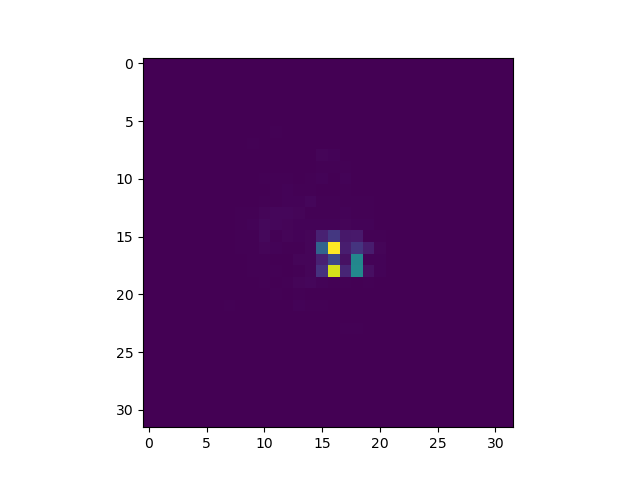
\includegraphics[width=.7\linewidth]{1450_poison_lrp.png}
			\caption{Zugehörige Heatmap bezüglich der Klasse 'Höchstgeschwindigkeit: 80km/h'}
			
		\end{subfigure}
		\caption{(Optischer) Vergleich von korrumpiertem Datenpunkt und berechnter Heatmap.}
		\label{vergleich_original_lrp}
	\end{figure}
	\subsection{Implementierung}
	
	\subsubsection{Tensorflow}
	\subsubsection{pytorch}
	
	\textbf{Allgemeines Tutorial}:\footnote{\url{https://git.tu-berlin.de/gmontavon/lrp-tutorial}}\\ pytorch-LRP für VGG16 wird vorgestellt.\\
	
	
	\noindent \textbf{GiorgioML}\footnote{\url{https://giorgiomorales.github.io/Layer-wise-Relevance-Propagation-in-Pytorch/}}:\\
	Alternative pytorch-Implementierung basierend auf Tensorflow paper.\\
	
	\noindent \textbf{moboehle}\footnote{\url{https://github.com/moboehle/Pytorch-LRP}}:\\
	Der code entstand im Rahmen der Forschungsarbeit \cite{lrp_alzheimer}, in der eine Alzheimer-Festellung aufgrund von Bilddaten(scans?) vorgenommen wird. Framework leicht anpasspar. Benutzt pytorch hooks. 
	\noindent Unterstützte Netzwerkschickten\footnote{\url{https://github.com/moboehle/Pytorch-LRP/blob/master/inverter_util.py}}:\\
	\begin{comment}
		
	
	\noindent $allowed\_pass\_layers = (torch.nn.BatchNorm1d, torch.nn.BatchNorm2d,\\
	torch.nn.BatchNorm3d,
	torch.nn.ReLU, torch.nn.ELU, Flatten,
	torch.nn.Dropout,\\ torch.nn.Dropout2d,
	torch.nn.Dropout3d,
	torch.nn.Softmax,
	torch.nn.LogSoftmax,
	torch.nn.Sigmoid)$\\
	\end{comment}
	\begin{lstlisting}[language=Python, caption=Verfügbare Schichten und Aktivierungsfunktionen]
	torch.nn.BatchNorm1d, 
	torch.nn.BatchNorm2d
	torch.nn.BatchNorm3d,
	torch.nn.ReLU, 
	torch.nn.ELU, 
	Flatten,
	torch.nn.Dropout,
	torch.nn.Dropout2d,
	torch.nn.Dropout3d,
	torch.nn.Softmax,
	torch.nn.LogSoftmax,
	torch.nn.Sigmoid
	
	\end{lstlisting}
	\noindent \textbf{fhvilshoj}\footnote{\url{https://github.com/fhvilshoj/TorchLRP}}:\\
	
	
	
	\noindent LRP für linear und Convolutional layers
	
	\begin{itemize}
		\item Die Klassen
	
	torch.nn.Sequential, torch.nn.Linear und torch.nn.Conv2d werden erweitert, um autograd für die Berechnung der Relevanzen zu berechnen.
	
		\item Ausgabe der Relevanzen von Zwischenschichten ist möglich
		\item: Implementierte Regeln: epsilon Regeln mit epsilon=1e-1, gamma-regel mit gamma=1e-1. alphabeta-Reagel mit a1b0 und a2b1
		\item Netz muss hier umgeschrieben werden, sodass die Anwendung des Algorithmus möglich wird.
	\end{itemize}

\begin{lstlisting}[language=Python, caption=Implementierte Regeln fhvilshoj]

	conv2d = {
		"gradient":             F.conv2d,
		"epsilon":              Conv2DEpsilon.apply,
		"gamma":                Conv2DGamma.apply,
		"gamma+epsilon":        Conv2DGammaEpsilon.apply,
		"alpha1beta0":          Conv2DAlpha1Beta0.apply,
		"alpha2beta1":          Conv2DAlpha2Beta1.apply,
		"patternattribution":   Conv2DPatternAttribution.apply,
		"patternnet":           Conv2DPatternNet.apply,
	}
	
\end{lstlisting}
	
	\noindent \textbf{Zennit}:\footnote{\url{https://github.com/chr5tphr/zennit}}
	Zennit (Zennit explains neural networks in torch) 
	\begin{itemize}
		\item Modell wird mithilfe eines Canonizers so aufbereitet, dass LRP möglich wird
		\item Backward pass wird modifiziert, um Heatmaps zu erhalten.
		\item VGG- und ResNet-Beispiel
	\end{itemize}
	\section{Detektion von Poisoning-Angriffen basierend auf LRP} \label{chapter_algorithm}
	\subsection{Idee}
	Die Idee zur Detektion von Poisoning-Angriffen besteht aus den folgenden Schritten:
	
	\begin{itemize}
		\item Berechnung der Heatmaps mit Hilfe der LRP
		\item Berechnung einer Distanzmatrix basierend auf $L^2-$ oder GMW-Distanz
		\item Spektrale Relevanzanalyse (Bestimmung der verschiedenen Cluster innerhalb einer Klasse)
	\end{itemize}

	\noindent  \textbf{Bemerkung:} Anstatt das Clustering nur auf den Heatmaps durchzuführen, könnten die LRP-Ausgaben und/oder Aktivierungen bestimmer NEtzwerkschichten hinzugenommen werden.\\
	
	The theory of optimal transport generalizes thatintuition in the case where, instead of moving only one item at a time, one is concernedwith the problem of moving simultaneously several items (or a continuous distributionthereof) from one configuration onto another.\cite{computationalOT}
	\subsection{Verwendete Distanzen \& Approximationen}
	
	Um die Struktur innerhalb einer Klasse zu analysieren, benötigen wir eine Metrik.
	Anhand dieser wird abhängig von den Heatmps einer Klasse eine Affinitätsmatrix berechnet, die dann anschließend zur Berechnung der Spektralen Einbettung als wichtigster Schritt von SpRAy verwendet wird. Wir wollen dazu die im Folgenden vorgestellten Metriken verweden.\\
	Wie in \cite{imagenet_unhansed_v1} summieren wir über die Farbkanäle, um einen einzelnen Relevanzwert pro Pixelpunkt zu erhalten. Wir benötigen also eine Metrik zur Berechnung der Distanz zwischen 32x32 großen Heatmaps.\\
	Wir normalisieren die Relevanzen zusätzlich auf das Intervall $[0,1]$.
	
	\begin{definition}[Distanz]
		Eine \emph{Distanz}
	\end{definition}
	\begin{definition}
		Eine \emph{Metrik}
	\end{definition}[Metrik]

	
	
	\subsubsection{Euklidische Distanz} \label{l2dist}
	Für den Fall der euklidischen Distanz schreiben wir die Relevanzwerte pro Pixel als Vektor und berechnen die Distanz zweier Heatmaps x und y wie folgt\footnote{\url{https://paulrohan.medium.com/euclidean-distance-and-normalization-of-a-vector-76f7a97abd9}}:
	$$ d_{x,y} = \sqrt{\sum_{i=1}^{32 * 32}{(x_i -y_i)^2}}.$$
	
	\subsubsection{Gromov-Hausdorff-Distanz}
	
	\begin{definition}[Hausdorff-Distanz]
		Sei $(M,d)$ ein metrischer Raum.
		Für 
		Seien $X,Y \subset (M,d)$ definieren wir die \emph{Hausdorff-Distanz} $d_H(X,Y)$ als
		
		\begin{equation}
			d_H(X,Y) = \max \lbrace \sup_{x \in X} \inf_{y \in Y} d(x,y), \sup_{y \in Y} \inf_{x \in Y} d(x,y) \rbrace .
		\end{equation} 
		
	\end{definition}

	%\begin{figure}
	%	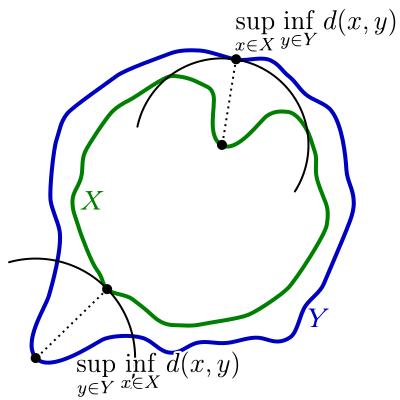
\includegraphics{Hausdorff_distance_sample}
	%\end{figure}
	\begin{definition}[Metrischer Maßraum]
	Ein \emph{metrischer Maßraum} ist ein Tripel $(X,d_x,\mu_X)$, wobei $(X,d_X)$ ein metrischer Raum und $\mu_X$ ein borelsches W-Maß auf $X$ ist.
	\end{definition}

	\begin{definition}[Correspondance]
		content...
	\end{definition}

	\begin{definition}[Kopplung]
	Seien 
	\end{definition}
	
	Seien $(X,d_X)$ und $(Y,d_Y)$ zwei metrische Räume. Wir betrachten im Folgenden die Abbildung
	\begin{equation}
		\Gamma_{X,Y}: (X\times Y) \times (X \times Y) \to \mathbb{R^{+}},
	\end{equation}
	gegeben durch
	
	$\Gamma_{X,Y}(x,y,x',y'):= |d_X(x,x') - d_Y(y,y')|$.
	
	\begin{definition}[Gromov-Hausdorff-Distanz]
	Für die metrischen Räume $(X,d_X)$ und $(Y,d_Y)$ ist die \emph{Gromov-Hausdorff-Distanz} definiert als
	\begin{equation}
		d_{\mathcal{G}\mathcal{H}} = \frac{1}{2}\inf_{R}||\Gamma_{X,Y}||_{L^\infty(R \times R)}.
	\end{equation}
	\end{definition}
	
	
	
	\subsection{Kantorovichs Optimal Transport Problem}
	
	\subsubsection{Gromov-Wasserstein-Distanz}
	
	\subsubsection{Entropisch Regularisierte Gromov-Wasserstein-Distanz}
	Entropic Regularization of Optimal Transport \cite{computationalOT}
	Mehrere Möglichkeiten einer Regularisierung der GW-Distanz\footnote{\url{https://www.youtube.com/watch?v=cPVMHWF8fmE&t=2532s}}:
	\begin{itemize}
		\item first\\
		\item second \\
		\item Entropy
	\end{itemize} 
	
	Optimal Transport: Regularization and Applications
	\footnote{\url{https://www.otra2020.com/schedule}}
	Python Optimal Transport Toolbox\footnote{\url{https://pythonot.github.io/quickstart.html}}\footnote{\url{https://pythonot.github.io/auto_examples/gromov/plot_gromov.html}}
	
	Matlab code\footnote{\url{https://github.com/gpeyre/2016-ICML-gromov-wasserstein}} zum Paper \cite{gwd_averaging_kernels}.
	Implementierung ist mittlerweile auch in der Python Optimal Transport toolbox verfügbar(s.o.).
	
	\subsubsection{Wasserstein Baryzentren}
	
	\subsubsection{Verallgemeinerung}
	Verallgemeinerung auf beliebige  Matrizen C, d.h. diese Distanzmatrizen müssen nicht notwendigerweise positiv sein und die Dreiecksungleichung erfüllen.
	
	Definiere die verallgemeinerte Gromov-Wasserstein-Distanz (vGWD) wie folgt:
	
	\begin{definition}[Verallgemeinerte Gromov-Wasserstein-Distanz]
		Seien zwei gewichtete Ähnlichkeitsmatrizen $(C,p) \in \mathbb{R}^{N_1 \times N_1} \times \Sigma_{N_1}$ und $(\bar{C},q) \in \mathbb{R}^{N_2 \times N_2} \times \Sigma_{N_2}$ gegeben. Sei $T$ eine Kopplung zwischen den beiden Räumen, auf denen die Matrizen $C$ und $\bar{C}$ definiert sind. Sei $L$ eine Fehlerfunktion. Dann definieren wir die verallgemeinerte Gromov-Wasserstein-Distanz als
		\begin{equation}
			vGw(C, \bar{C}, p, q) := \min_{T \in \mathcal{C}_{p, q}}{\mathcal{\varepsilon}_{C,\bar{C}}(T)},
		\end{equation}
		wobei gilt $\mathcal{\varepsilon}_{C,\bar{C}}(T) := \sum_{i,j,k,l}{L(C_{i,k}, \bar{C}_{j,l})T_{i,j}T_{k,l}}.$
		
	\end{definition}

	Häufig verwendete Fehlerfunktionen sind die quadratische Fehlerfunktion $L(a,b) = L_2(a,b) := \frac{1}{2}|a-b|^2$ und die Kullback-Leibler-Divergenz $L(a,b)  = KL(a|b) := a\log(a/b) -a+b$.
	
	Diese Definition der Gromov-Wasserstein-Distanz verallgemeinert die Version in \cite{gwd_averaging_kernels}, da hier beliebige Fehlerfunktionen betrachtet werden.\\
	
	Für L=L2 zeigt Memoli,2011, dass GW1/2 eine Distanz definiert.
	\subsection{Spektrales Clustering}
	Wir folgen \cite{spectralClustering_tut}.
	Gegeben:Datenpunkte $x_i, ..., x_n$ sowie eine Größe $s = s_{ij} \in \mathbb{R}^{+}$, die einen paarweisen Zusammenhang der einzelnen Punkte beschreiben.
	
	Ziel: Aufteilen der Punkte in verschiedene Cluster, sodass sich Punkte innerhalb eines Clusters ähnlich bezüglich $s$ sind.
	
	Alternative Repräsentation der Daten mithilfe eines Ähnlichkeitsgraphen $G=(V,E)$ möglich.
	
	Umformulierung des Clustering-Problems mithilfe des Ähnlichkeitsgraphen: Finde Pertitionierung des Graphen, sodass die Kanten-Gewichte innerhalb einer Gruppe niedrig (niedriges Gesamtgewicht?) und außerhalb einer Gruppe große sind.\\
	
	
	Graph-Notationen:\\
	
	Verschiedene Konstruktionsmöglichkeiten von Ähnlichkeitsgraphen:
	
	\begin{itemize}
		\item $\varepsilon$-Nachbarschaft-Graph\\
		\item kNN-Graph\\
		\item fully connected graph
	\end{itemize}

	\subsection{k-means / k-means++ -Clustering}
	
	Beispiel-Implementierung\footnote{\url{https://towardsdatascience.com/k-means-implementation-in-python-and-spark-856e7eb5fe9b}}\\
	\\
	Baryzentrische Koordinaten \footnote{\url{https://de.wikipedia.org/wiki/Baryzentrische_Koordinaten}}
	\subsection{Anwendung auf unterschiedliche Poisoning-Angriffe} \label{chapter_results} \label{chapter_experiments}
	\noindent \textbf{Berechnung der Relevanzen}:\\
	
	\noindent Wir berechnen die Relevanzen jedes einzelenen Eingabebildes klassenweise, d.h. besitzt eine Eingabe das Label y, so berechnen auf einem trainierten Netzwerk, für jeden Pixelwert der Eingabe, wie relevant dieser für die Ausgabe f(x) = y ist.\\
	Wir summieren über die Farbaxen des Bildes, um einzelne Relevanzen pro Pixelpunkt zu erhalten.\\
	Für die Berechnung der Relevanzen benutzen wir eine modifizierte Version des im Rahmen von \cite{lrp_alzheimer} entstandenen Programmcodes\footnote{\url{https://github.com/moboehle/Pytorch-LRP}}.\\
	\\
	\noindent \textbf{Vorverarbeitung der Relevanzen:}\\
	In \cite{unmaskingCH} wird anschließend ein Sum-Pooling auf die Relevanzen angewendet, um eine Dimensionsreduktion zu erhalten. Wie in \cite{imagenet_unhansed_v1} verzichten wir auf eine weitere Dimensionsreduktion, da wir nur relativ kleine Relevanzen der Größe $32x32$ verarbeiten.	\\
	
	Für eps=5e-2 liegen beide barycentren identisch weit weg. Probiere nun eps=5e-3
	
	\noindent \textbf{Berechnung der Distanzen und Aufstellen einer Affinitätsmatrix:}\\
	
	Wir berechnen zunächst eine Distannzmatrix, die die paarweisen Distanzen aller Heatmaps einer Klasse enthält.	
	
	Für die Berechnung der euklidischen Distanz betrachten wir Heatmaps $x,y$ der Größe $32x32$ als Elemente $x,y \in \mathbb{R}^{32*32}$ Die Distanz lässt sich dann wie in \autoref{l2dist} berechnen.\\
	
	Die Gromov-Wasserstein-Distanz lässt sich wie in \cite{gwd_averaging_kernels} angegeben berechnen. \\
	
	Barycenters Definition und Vergleich zum euklidischen Raum \cite{bary_wasserstein_space}
	
	In einer Affinitätsmatrix oder Ähnlichkeitsmatrik sind die \\
	
	\noindent \textbf{Berechnung Spektralen Einbettung:}\\
	
	\noindent \textbf{Dimensionsreduktion vor dem Clustering ?!}\\
	
	In \cite{AC} wird beispielsweise eine Dimensionsreduktion mit PCA durchgeführt.
	
	\noindent \textbf{k-Means-Clustering:}\\
	\begin{remark}
		In \cite{imagenet_unhansed_v1} Kapitel '2.3. Fisher Discriminant Analysis for Clever Hans
		identification' wird ein Verfahren vorgestellt, mit dem verdächtige Klassen indentifiziert werden können. Für diese würde man anschließend das obige Verfahren durchführen
	\end{remark}
	\subsubsection{Standard Poisoning-Angriffe}
	
	
	=> Did save Model - incv320epochsnormalized - at epoch: 19
	=>	[19] loss: 0.125, accuracy: 96.514%
	=>	Accuracy of validation Dataset: 98.491% 
	
	=>	FINISHED TRAINING
	loss on test dataset: 3.284087032527311
	Accuracy of test Dataset: 0.919 
	
	BDSR classwise:
	[nan nan  1. nan nan nan nan nan nan nan nan nan nan nan nan nan nan nan
	nan nan nan nan nan nan nan nan nan nan nan nan nan nan nan nan nan nan
	nan nan nan nan nan nan nan]
	
	Performance of poisoned net on unpoisoned training data:
	loss on test dataset: 0.15269652156995248
	Accuracy of test Dataset: 0.961 \\

	
	\noindent \textbf{Performance auf nicht korrumpierten Daten:}\\
	=>	FINISHED TRAINING
	loss on test dataset: 0.15834395289583986
	Accuracy of test Dataset: 0.968 \\
	
	%BDSR classwise:Histogramm
	%[nan nan nan nan nan nan nan nan nan nan nan nan nan nan nan nan nan nan$(C,p) \in \mathbb{R}^{N_1 \times \N_1} \times \Sigma_{N_1}$
	%nan nan nan nan nan nan nan nan nan nan nan nan nan nan nan nan nan nan
	%nan nan nan nan nan nan nan]
	%Performance of poisoned net on unpoisoned training data:
	%loss on test dataset: 0.2061727911354566
	%Accuracy of test Dataset: 0.951 
	
	%: Warum gibts bei den beiden oberen Auswertungen %einen Unterschied?
	
	\noindent \textbf{Spektralanalyse:}
	
	\begin{figure}[h]
	\begin{center}
		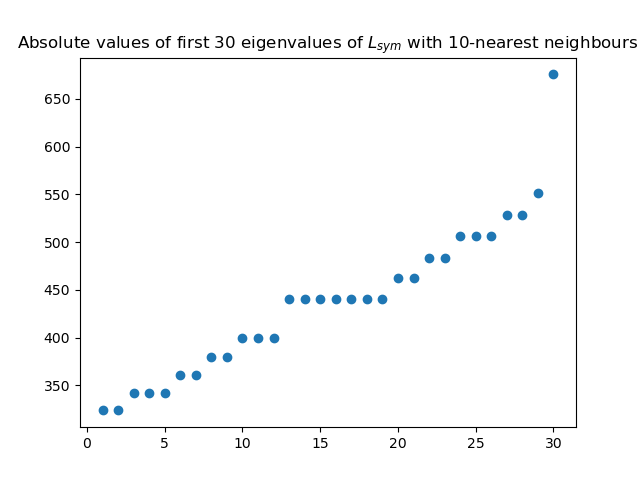
\includegraphics[width=0.5\textheight]{specClustering_l2_k10.png}
		\caption{Ergebnis des spektralen Clusterings unter Verwendung der Euklidischen Distanz und k=10 Nachbarn}
	\end{center}
	\end{figure}
	
	\noindent \textbf{Clustering(euklidisch):}
	$(tn, fp, fn, tp) = 1650, 0, 386, 427)$\\
	\\
	\noindent \textbf{Clustering(GWD):}
	\begin{figure}[h]
		\begin{center}
			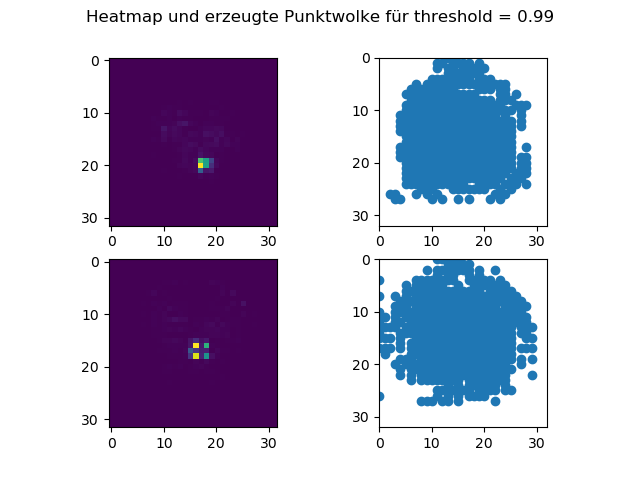
\includegraphics[width=0.5\textheight]{HeatmapPunktwolke99.png}
			\caption{Auswahl der relevantesten Pixel (bis zu $99\%$ der Gesamtmasse) zweier Heatmaps}
		\end{center}
	\end{figure}

\begin{figure}[h]
	\begin{center}
		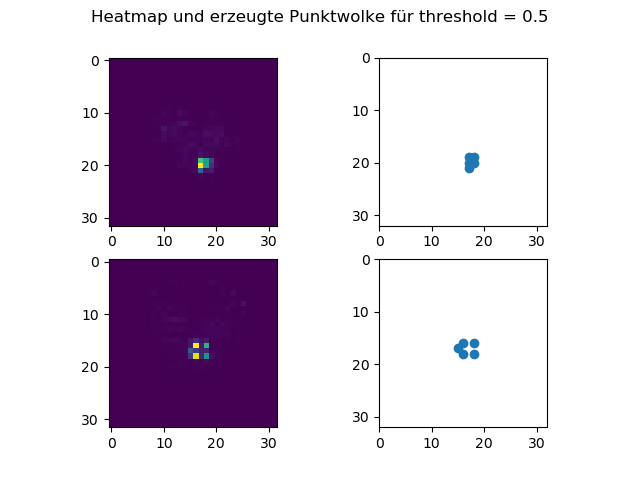
\includegraphics[width=0.5\textheight]{HeatmapPunktwolke50.png}
		\caption{Auswahl der relevantesten Pixel (bis zu $50\%$ der Gesamtmasse) zweier Heatmaps}
	\end{center}
\end{figure}

	\begin{figure}[h]
		\begin{center}
			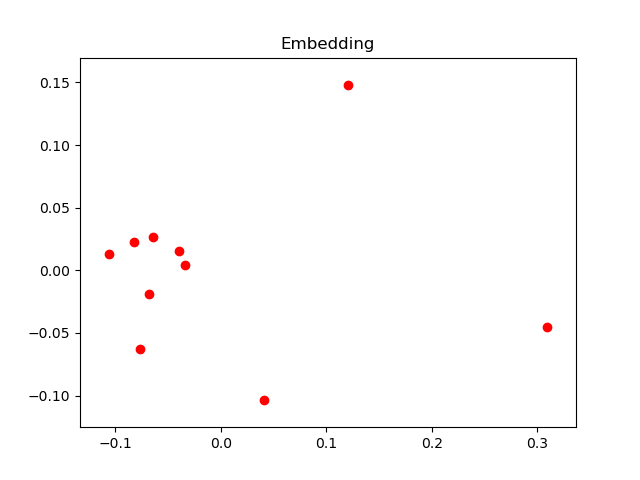
\includegraphics[width=0.5\textheight]{bary_embedding99.png}
			\caption{Einbettung des Baryzentrums mithilfe von Multidimensionaler Skalierung(MDS) bei der Wahl von $99\%$ der Gesamtmasse}
		\end{center}
	\end{figure}


	n=5
	Berechnung der Distanzen:
	Clustering:  [1. 0. 1. 0. 1.]
	--- 379.38680505752563 seconds ---
	
	Berechnung von 2 Baryzentren
	--- 725.2780563831329 seconds ---
	
	n=25
	Berechnung der Distanzen:
	Clustering:  [1. 0. 1. 0. 1. 0. 1. 0. 0. 1. 1. 0. 0. 0. 1. 0. 0. 0. 1. 0. 0. 1. 0. 1.
	1.]
	--- 1860.5442748069763 seconds ---
	
	Berechnung von zwei Baryzentren
	--- 2443.7355489730835 seconds ---
	
	n=50
	Berechnung der Distanzen:
	--- 1956.3804433345795 seconds ---
	
	Berechnung von zwei Barycentern:
	--- 5670.336745262146 seconds ---
	
	15 Prozenmt 3x3 Sticker
	=> Did save Model - SAincV3s315 - at epoch: 50
	=>	[50] loss: 0.060, accuracy: 98.405%
	EarlyStopping counter: 20 out of 20
	Early stopping
	=>	FINISHED TRAINING
	loss on test dataset: 3.736420426017416
	Accuracy of test Dataset: 0.911 
	
	BDSR classwise:
	[nan nan  1. nan nan nan nan nan nan nan nan nan nan nan nan nan nan nan
	nan nan nan nan nan nan nan nan nan nan nan nan nan nan nan nan nan nan
	nan nan nan nan nan nan nan]
	Performance of poisoned net on unpoisoned training data:
	loss on test dataset: 0.1822473893020984
	Accuracy on test Dataset: 0.961 
	
	\begin{center}
		
	\end{center}
	
	
	\subsubsection{Label-konsistente Poisoning-Angriffe}
	\section{Vergleich mit anderen Verfahren} \label{chapter_comparisons}
	\subsection{Activation Clustering}
	\subsection{Räumliche Transformationen}
	\begin{itemize}
		\item ASR ist sehr stark vom Ort des Triggers abhängig.
		\item Ort des Triggers kann nicht direkt geändert werden.
		\item Benutze Transformationen(Flipping, Scaling), um den Trigger wirkungslos zu machen.
		\item Somit kann die ASR während der Inferenz verringert werden. Es lässt sich aber keine Auussage darüber treffen, ob ein Angriff vorliegt
	\end{itemize}
	
	\section{Weitere mögliche Schritte} \label{chapter_weitereSchritte}
	\begin{itemize}
		\item Automatische Platzierung des Auslösers an fest gewählter Position auf dem Verkehrsschild anstatt zufälligem Platzieren in einem Fenster mit vorher festgelegter Größe. In \cite{badnets} wird  Faster-RCNN (F-RCNN) zur Klassifikation des LISA-Datensatzes\footnote{\url{http://cvrr.ucsd.edu/LISA/lisa-traffic-sign-dataset.html}} benutzt. Es ist die Aufgabe, die Verkehrsschilder in die 3 Superklassen Stoppschild, Geschwindigkeitsbegrenzung und Warnschild einzuteilen. Der Datensatz enthält zudem die BoundingBoxen, sodass der Auslöser genauer angebracht werden kann.
		\item Verbesserte Version der Layer-wise Relevance Propagation
		\item Untersuchung anderer Verfahren, die die Interpretierbarkeit ermöglichen, beispielsweise: VisualBackProp: efficient visualization of CNNs\footnote{\url{https://arxiv.org/abs/1611.05418}}
		\item Vergleich mit Cifar-10/Cifar-100 Datensatz\footnote{\url{https://www.cs.toronto.edu/~kriz/cifar.html}}\footnote{\url{https://www.cs.toronto.edu/~kriz/learning-features-2009-TR.pdf}}
	\end{itemize}


	\section{Zusammenfassung} \label{chapter_conclusion}
	
	\printglossaries
	\newpage
	\appendix
	\section{Verwendete Netzwerke}
	\subsection{Net}
	
	\begin{lstlisting}[language=Python, caption=Kleines Netzwerk]
	
	class Net(nn.Module):
	
		def __init__(self, ):
			super(Net, self).__init__()
			self.size = 64 * 4 * 4
			self.conv1 = nn.Conv2d(in_channels=3, out_channels=12, kernel_size=5, padding=2)
			self.pool = nn.MaxPool2d(kernel_size=2, stride=2)
			self.conv1_in = nn.InstanceNorm2d(12)
			self.conv2 = nn.Conv2d(in_channels=12, out_channels=32, kernel_size=5, padding=2)
			
			self.conv2_bn = nn.BatchNorm2d(32)
			
			self.conv3 = nn.Conv2d(in_channels=32, out_channels=64, kernel_size=5, padding=2)
			
			self.fc1 = nn.Linear(self.size, 256)
			self.fc1_bn = nn.BatchNorm1d(256)
			self.fc2 = nn.Linear(256, 128)
			self.fc3 = nn.Linear(128, 43)
		
	
		def forward(self, x):
			x = self.pool(F.relu(self.conv1_in(self.conv1(x))))
			x = self.pool(F.relu(self.conv2_bn(self.conv2(x))))
			x = self.pool(F.relu(self.conv3(x)))
			x = x.view(-1, self.size)
			x = F.relu(self.fc1_bn(self.fc1(x)))
			x = F.dropout(x)
			xx = F.relu(self.fc2(x))
			x = F.dropout(xx)
			x = self.fc3(x)
			
			return x, xx
	
	\end{lstlisting}
	
	\begin{lstlisting}[language=Python, caption=Einfachere Version von Inception v3]
		InceptionNet3(
		(features): Sequential(
		(0): InceptionA(
		(parallel_dummyA): New_parallel_chain_dummy()
		(conv1x1): BatchConv(
		(conv): Conv2d(3, 64, kernel_size=(1, 1), stride=(1, 1))
		(bn): BatchNorm2d(64, eps=1e-05, momentum=0.1, affine=True, track_running_stats=True)
		(relu): ReLU()
		)
		(parallel_dummyB): New_parallel_chain_dummy()
		(conv5x5_1): BatchConv(
		(conv): Conv2d(3, 48, kernel_size=(1, 1), stride=(1, 1))
		(bn): BatchNorm2d(48, eps=1e-05, momentum=0.1, affine=True, track_running_stats=True)
		(relu): ReLU()
		)
		(conv5x5_2): BatchConv(
		(conv): Conv2d(48, 64, kernel_size=(5, 5), stride=(1, 1), padding=(2, 2))
		(bn): BatchNorm2d(64, eps=1e-05, momentum=0.1, affine=True, track_running_stats=True)
		(relu): ReLU()
		)
		(parallel_dummyC): New_parallel_chain_dummy()
		(conv3x3dbl_1): BatchConv(
		(conv): Conv2d(3, 64, kernel_size=(1, 1), stride=(1, 1))
		(bn): BatchNorm2d(64, eps=1e-05, momentum=0.1, affine=True, track_running_stats=True)
		(relu): ReLU()
		)
		(conv3x3dbl_2): BatchConv(
		(conv): Conv2d(64, 96, kernel_size=(3, 3), stride=(1, 1), padding=(1, 1))
		(bn): BatchNorm2d(96, eps=1e-05, momentum=0.1, affine=True, track_running_stats=True)
		(relu): ReLU()
		)
		(conv3x3dbl_3): BatchConv(
		(conv): Conv2d(96, 96, kernel_size=(3, 3), stride=(1, 1), padding=(1, 1))
		(bn): BatchNorm2d(96, eps=1e-05, momentum=0.1, affine=True, track_running_stats=True)
		(relu): ReLU()
		)
		(parallel_dummyD): New_parallel_chain_dummy()
		(pool): MaxPool2d(kernel_size=3, stride=1, padding=1, dilation=1, ceil_mode=False)
		(pool1x1): BatchConv(
		(conv): Conv2d(3, 32, kernel_size=(1, 1), stride=(1, 1))
		(bn): BatchNorm2d(32, eps=1e-05, momentum=0.1, affine=True, track_running_stats=True)
		(relu): ReLU()
		)
		(parallel_dummyE): New_parallel_chain_dummy()
		(cat): Cat()
		)
		(1): MaxPool2d(kernel_size=2, stride=2, padding=0, dilation=1, ceil_mode=False)
		(2): BatchConv(
		(conv): Conv2d(256, 256, kernel_size=(2, 2), stride=(1, 1))
		(bn): BatchNorm2d(256, eps=1e-05, momentum=0.1, affine=True, track_running_stats=True)
		(relu): ReLU()
		)
		(3): MaxPool2d(kernel_size=2, stride=2, padding=0, dilation=1, ceil_mode=False)
		(4): BatchConv(
		(conv): Conv2d(256, 256, kernel_size=(2, 2), stride=(1, 1))
		(bn): BatchNorm2d(256, eps=1e-05, momentum=0.1, affine=True, track_running_stats=True)
		(relu): ReLU()
		)
		(5): MaxPool2d(kernel_size=2, stride=2, padding=0, dilation=1, ceil_mode=False)
		(6): BatchConv(
		(conv): Conv2d(256, 256, kernel_size=(2, 2), stride=(1, 1))
		(bn): BatchNorm2d(256, eps=1e-05, momentum=0.1, affine=True, track_running_stats=True)
		(relu): ReLU()
		)
		(7): MaxPool2d(kernel_size=2, stride=2, padding=0, dilation=1, ceil_mode=False)
		)
		(classifiers): Sequential(
		(0): Linear(in_features=256, out_features=256, bias=True)
		(1): ReLU(inplace=True)
		(2): Dropout(p=0.5, inplace=False)
		(3): Linear(in_features=256, out_features=128, bias=True)
		(4): ReLU(inplace=True)
		(5): Dropout(p=0.5, inplace=False)
		(6): Linear(in_features=128, out_features=43, bias=True)
		)
		)
	\end{lstlisting}
	Aufbau dieses Netzwerkes:
	 1. Inception-Modul
	 2. [pool1, batchConv1, pool2, batchConv2, pool3, batchConv3, pool4]
	 3. Drei Lineare Schichten mit ReLu und Dropout dazwischen
	
	Im Unterschied zum offiziellen Inception Netz(v1v2v3) gibt es in dieser 
	 vereeinfachten Versionn keinen "stem" aus convs, 
	 es geht direkt mit InceptionA los.
	
	 Wie ähnlich sind sich InceptionA(hier) und das offizielle InceptionA-Modul?
	\begin{lstlisting}[language=Python, caption=Reversed Model incv3]
	
	[Linear(in_features=128, out_features=43, bias=True), 
	Dropout(p=0.5, inplace=False), 
	ReLU(inplace=True), 
	Linear(in_features=256, out_features=128, bias=True), 
	Dropout(p=0.5, inplace=False), 
	ReLU(inplace=True), 
	Linear(in_features=256, out_features=256, bias=True), 
	MaxPool2d(kernel_size=2, stride=2, padding=0, dilation=1, ceil_mode=False), 
	ReLU(), 
	BatchNorm2d(256, eps=1e-05, momentum=0.1, affine=True, track_running_stats=True), Conv2d(256, 256, kernel_size=(2, 2), stride=(1, 1)), 
	MaxPool2d(kernel_size=2, stride=2, padding=0, dilation=1, ceil_mode=False), 
	ReLU(), 
	BatchNorm2d(256, eps=1e-05, momentum=0.1, affine=True, track_running_stats=True), Conv2d(256, 256, kernel_size=(2, 2), stride=(1, 1)), 
	MaxPool2d(kernel_size=2, stride=2, padding=0, dilation=1, ceil_mode=False), 
	ReLU(), BatchNorm2d(256, eps=1e-05, momentum=0.1, affine=True, track_running_stats=True), 
	Conv2d(256, 256, kernel_size=(2, 2), stride=(1, 1)), 
	MaxPool2d(kernel_size=2, stride=2, padding=0, dilation=1, ceil_mode=False),
	
	[[Conv2d(3, 64, kernel_size=(1, 1), stride=(1, 1)), 
	BatchNorm2d(64, eps=1e-05, momentum=0.1, affine=True, track_running_stats=True), ReLU()], 
	
	[Conv2d(3, 48, kernel_size=(1, 1), stride=(1, 1)), 
	BatchNorm2d(48, eps=1e-05, momentum=0.1, affine=True, track_running_stats=True), ReLU(), Conv2d(48, 64, kernel_size=(5, 5), stride=(1, 1), padding=(2, 2)), BatchNorm2d(64, eps=1e-05, momentum=0.1, affine=True, track_running_stats=True), ReLU()], 
	
	[Conv2d(3, 64, kernel_size=(1, 1), stride=(1, 1)), 
	BatchNorm2d(64, eps=1e-05, momentum=0.1, affine=True, track_running_stats=True), ReLU(), 
	Conv2d(64, 96, kernel_size=(3, 3), stride=(1, 1), padding=(1, 1)), 
	BatchNorm2d(96, eps=1e-05, momentum=0.1, affine=True, track_running_stats=True), ReLU(), 
	Conv2d(96, 96, kernel_size=(3, 3), stride=(1, 1), padding=(1, 1)), 
	BatchNorm2d(96, eps=1e-05, momentum=0.1, affine=True, track_running_stats=True), ReLU()], 
	
	[MaxPool2d(kernel_size=3, stride=1, padding=1, dilation=1, ceil_mode=False), Conv2d(3, 32, kernel_size=(1, 1), stride=(1, 1)), 
	BatchNorm2d(32, eps=1e-05, momentum=0.1, affine=True, track_running_stats=True), 
	ReLU()], 
	
	[Cat()]]]
	\end{lstlisting}
	\section{Parameter für Training und Einlesen der Daten}
	Die in \cite{CH} gewählten Parameter wären ein guter Ausgangspunkt.
	\section{Datensätze}
	\section{Programmcode}
	
	
	\verbatiminput{Netlayout.txt}
	
	\verbatiminput{InceptionNet3layout.txt}
	
	
	\newpage
	
	\printglossaries

	\newpage
	
	\bibliographystyle{apacite}
	
	\bibliography{bibfileMAlukasschulth}

	
	
\end{document}